%
% $Id: AttributeSet.java 15 2010-10-11 16:16:32Z justinkamerman $ 
%
% $LastChangedDate: 2010-10-11 13:16:32 -0300 (Mon, 11 Oct 2010) $ 
% 
% $LastChangedBy: justinkamerman $
%

\documentclass[10pt]{report}
\usepackage{graphicx}
\usepackage{setspace}			
\onehalfspacing

\title{CS6999 Programming Assignment 1}
\author{Justin Kamerman 3335272}
\date{\today}

\begin{document}
\maketitle
% No chapter numbers
\renewcommand*\thesection{\arabic{section}}

%----------------------------------------
% Assignment
%----------------------------------------
\section*{Assignment}
\begin{enumerate} 
\item Implement the Aho-Corasick string matching algorithm\cite{RefWorks:103} and test its performance for:
  \begin{itemize}
  \item 1000 blogs and  100 keywords
  \item 2,000 blogs and 100 keywords
  \item 4,000 blogs and 100 keywords
  \item 8,000 blogs and 100 keywords
  \item 16,000 blogs and 100 keywords
  \item 32,000 blogs and 100 keywords
  \end{itemize}
           
Repeat the experiments for 200 and 400 keywords.
      

\item Build an inverted index for 10, 000 blogs. Use 10 keywords to query the index to:
  \begin{itemize}
  \item Locate each keyword and retrieve their corresponding blogs.
  \item Show the intersection of every two keywords. For example, retrieve the document ID of the blogs that keywords 1 and 2 have occurred together at least once. Similarly, for keywords 1 and 3, ..., keywords 2 and 3, keywords 2 and 4, ...
    \item Similarly, show the intersection of every 3 keywords, 4 keywords, etc.
  \end{itemize}
  
\item Do a comparative analysis (time to build the index and time to retrieve) of the two methods.
\end{enumerate}

%----------------------------------------
% Aho-Corasick Algorithm
%----------------------------------------
\section{Aho-Corasick Algorithm}
\label{sec:ahocorasickalgorithm}
The Aho-Corasick string matching algorithm\cite{RefWorks:103} is a
kind of dictionary matching search algorithm that constructs a finite
state machine to scan for a given set of keywords. It is, in effect, a
reduced grammar regular expression parser described in
\cite{RefWorks:111}. In our search implementation, the finite state
machine is constructed from a list of keywords. Then the documents
of the test corpus are read from secondary storage and fed through the
finite state machine. As soon as a document is found to contain at
least one instance of each of a set of search terms, parsing of that document
ends.

The documents of the corpus are each stored in a disk file, named for
the identifier of the original blog extract. In an attempt to exploit
the fact that reading documents from disk is slower than state machine
scanning, the scan process uses a thread pool to read and parse
multiple documents concurrently. By expanding the thread pool, the
implementation is able to achieve higher CPU utilization and marginal
improvements in search times. However, the limits of the experiment
platform did not accommodate increasing the pool size to a point where
the added complexity and synchronization overhead were justified.


\subsection*{Implementation}
The Aho-Corasick algorithm are implemented by a Java
program. The only external dependency is on the Apache commons-cli
library for parsing commend line options. To that end, the program is
operated from the command line, taking options listed in table
~\ref{tab:ahocommandline}.  
\\
\begin{table}[h]
  \centering
  \begin{tabular}{ |l|p{10cm}|} 
    \hline
    Option & Description \\ \hline
    -d \<arg\>  &  Document directory \\ \hline
    -k \<arg\>  &  Keywords file \\ \hline
    -p \<arg\>  &  Thread pool size. Default is 10 \\ \hline
    -g          &  Generate DOT visualization of state machine \\ \hline
    -h          &  Print help message \\ \hline
  \end{tabular}
  \caption{Command line options for Aho-Corasick implementation}
  \label{tab:ahocommandline}
\end{table}
\\

The program implements various mechanism to facilitate
debugging. Throughout the code, log statements have been added using
the Java logging framework. The logging output is controlled for
individual classes via the \texttt{logging.properties} file which the
program read on start-up. In addition to logging, code was added to
generate Graphviz DOT\cite{RefWorks:110} output representing the state
machine created. A sample \textit{dot} file for the state machine
generated for the four keywords used in \cite{RefWorks:103}
(\textit{he, she, his, hers}), is shown below. The \textit{output
  function} for each state is shown in square braces and unlabelled
edges represent the \textit{failure function}.  The associated image
generated by DOT is shown in figure \ref{fig:dot}.


\begin{verbatim}
digraph G {
	0  [label="0 []", shape=circle];
	0 -> 3 [label="s"];
	0 -> 1 [label="h"];
	1  [label="1 []", shape=circle];
	1 -> 2 [label="e"];
	1 -> 6 [label="i"];
	1 -> 0 [color="red"];
	6  [label="6 []", shape=circle];
	6 -> 7 [label="s"];
	6 -> 0 [color="red"];
	7  [label="7 [his]", shape=circle];
	7 -> 3 [color="red"];
	2  [label="2 [he]", shape=circle];
	2 -> 8 [label="r"];
	2 -> 0 [color="red"];
	8  [label="8 []", shape=circle];
	8 -> 9 [label="s"];
	8 -> 0 [color="red"];
	9  [label="9 [hers]", shape=circle];
	9 -> 3 [color="red"];
	3  [label="3 []", shape=circle];
	3 -> 4 [label="h"];
	3 -> 0 [color="red"];
	4  [label="4 []", shape=circle];
	4 -> 5 [label="e"];
	4 -> 1 [color="red"];
	5  [label="5 [she, he]", shape=circle];
	5 -> 2 [color="red"];
}
\end{verbatim}

\begin{figure}
  \begin{center}
	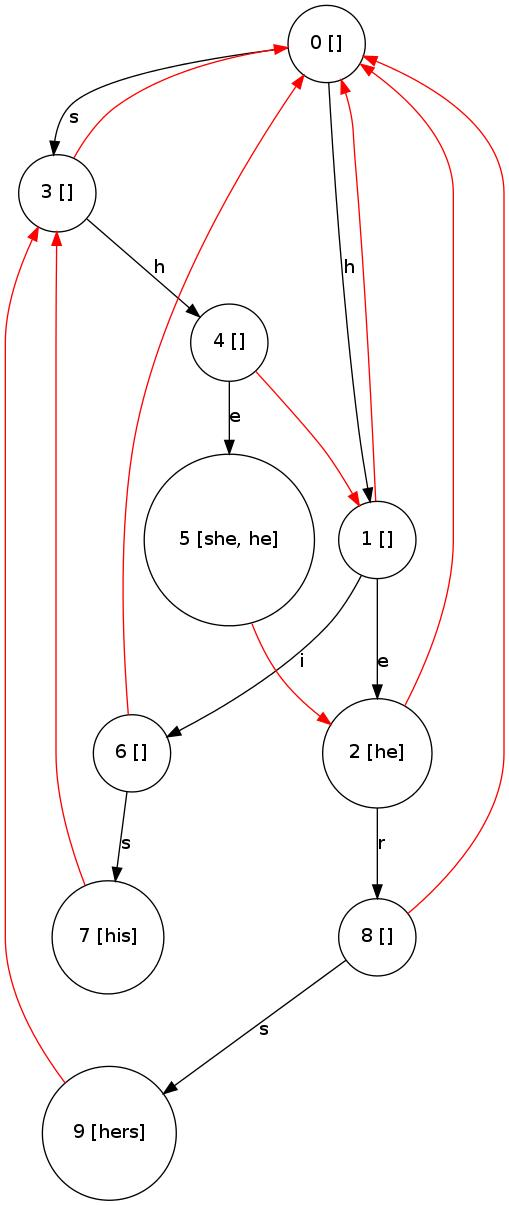
\includegraphics[width=!,height=0.90\textheight]{aho4}
  \end{center}
  \caption{Aho-Corasick state machine visualization generated by DOT}
  \label{fig:dot}
\end{figure} 

\begin{figure}
  \begin{center}
	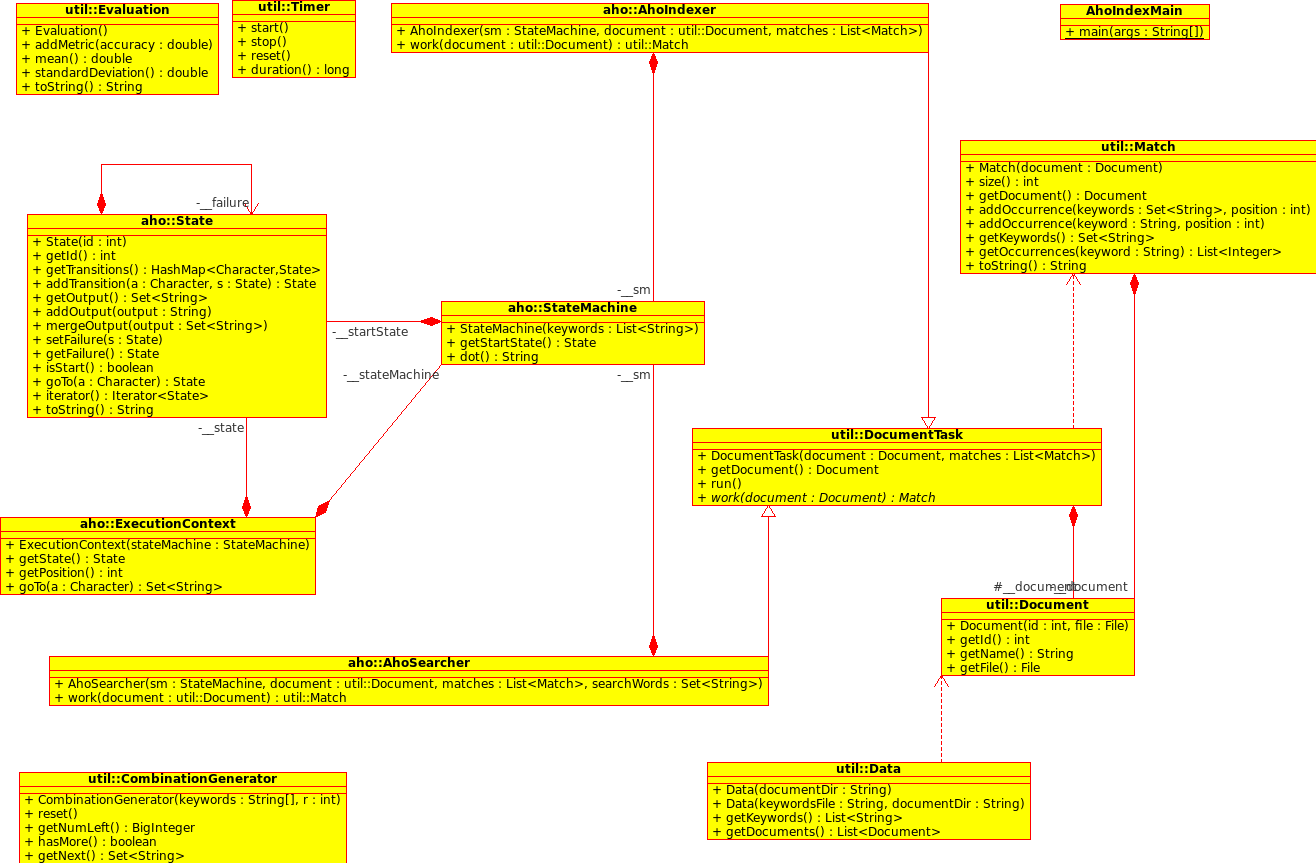
\includegraphics[angle=90,width=\textwidth,height=!]{ahouml}
  \end{center}
  \caption{Aho-Corasick Implementation UML class diagram}
  \label{fig:ahouml}
\end{figure} 

The implementation classes and their relationships are represented in
a UML class diagram in figure \ref{fig:ahouml}. Following is a brief
description of each class:

\begin{itemize}
\item \textbf{AhoIndexMain:} a driver class for the Aho-Corasick
  implementation. It performs the scanning tests and gathers data
  presented in this report. This class manages the thread pool used to
  parallelize the scanning process.

\item \textbf{AhoSearchMain:} a driver class for the Aho-Corasick
  implementation. It performs the search tests and gathers data
  presented in this report. This class manages the thread pool used to
  parallelize the search process.

\item \textbf{AhoIndexer:} manages the scanning of documents by the
  state machine. It presents an interface suitable for use by the
  thread pool.

\item \textbf{AhoSearcher:} manages the searching of documents by the
  state machine. It presents an interface suitable for use by the
  thread pool.

\item \textbf{CombinationGenerator:} this class generates the ${n
  \choose k}$ search term combinations required for the search
  evaluation. It borrows heavily from source code published by Michael
  Gilleland at Miriam Park Software.

\item \textbf{Evaluation:} a utility class for aggregating general
  test results and calculating means and standard deviations.

\item \textbf{ExecutionContext:} externalizes an execution path
  through a \texttt{StateMachine} so that the machine can be used
  concurrently by multiple threads.

\item \textbf{StateIterator:} utility class for iterating through all
  states of a \texttt{StateMachine}. Used in generating DOT
  visualization output.

\item \textbf{StateMachine:} represents the finite state machine
  created by the Aho-Corasick string matching
  algorithm\cite{RefWorks:103}.

\item \textbf{Data:} utility class for reading blog and keyword files
  from the filesystem.

\item \textbf{Document:} encapsulates document attributes.

\item \textbf{DocumentTask:} abstract class which enforces an
  interface suitable for use by the thread pool. Subclasses include
  \texttt{AhoSearcher} and \texttt{AhoIndexer}.

\item \textbf{LogFormatter:} is a helper class to format log messages.

\item \textbf{Match:} maps a \texttt{Document} to a set of keywords
  that occur in the document and their position with the document.

\item \textbf{Timer:} utility class for collecting execution times.
\end{itemize}


\subsection*{Results}
Various tests were conducted to characterize the performance of the
Aho-Corasick search algorithm:

\begin{itemize}
\item The time taken to construct the Aho-Corasick state machine was
  measured for different numbers of keywords. The results of this test
  is shown in figure \ref{fig:ahostatemachine} and construction time
  can easily be considered linear with respect to the number of
  keywords. This is consistent with \cite{RefWorks:103} which proves
  that the state machine construction algorithm is linearly
  proportional to the sum of the lengths of the keywords used to
  construct the state machine.

\item The time taken for the Aho-Corasick state machine to scan
  different sized corpora was measured. The test was repeated for
  various state machines, constructed using a 100, 200, and 400
  keyword set. The results of this test are shown on figure
  \ref{fig:ahoscan} and indicate that scan time is nearly linear with
  respect to the size of the corpus and independent of the number of
  keywords used to generate the state machine. This last result is
  consistent with \cite{RefWorks:103} which proves that the number of
  state transitions involved in processing an input string is
  independent of the number of keywords used to construct the state
  machine.

\item The time taken to search for different numbers of keywords was
  measured over different sized corpora. A set of ten keywords was
  selected randomly and the the corpora searched for ${n \choose k}$
  enumerated combinations thereof to obtain an average for a
  particular keyword set size. The results of this test are shown in
  figure \ref{fig:ahosearch} and indicate that search time is
  independent of the number of terms used in the search and linear
  with respect to the size of the corpus. This first result is
  surprising given that the search process exists as soon as a single
  instance of each search term is found. One would expect the number
  of documents scanned completely to increase as the number of search
  term increases. The small average document size and the fact that
  the search hit rate is low may account for this phenomenon.
\end{itemize}


\begin{figure}
  \begin{center}
	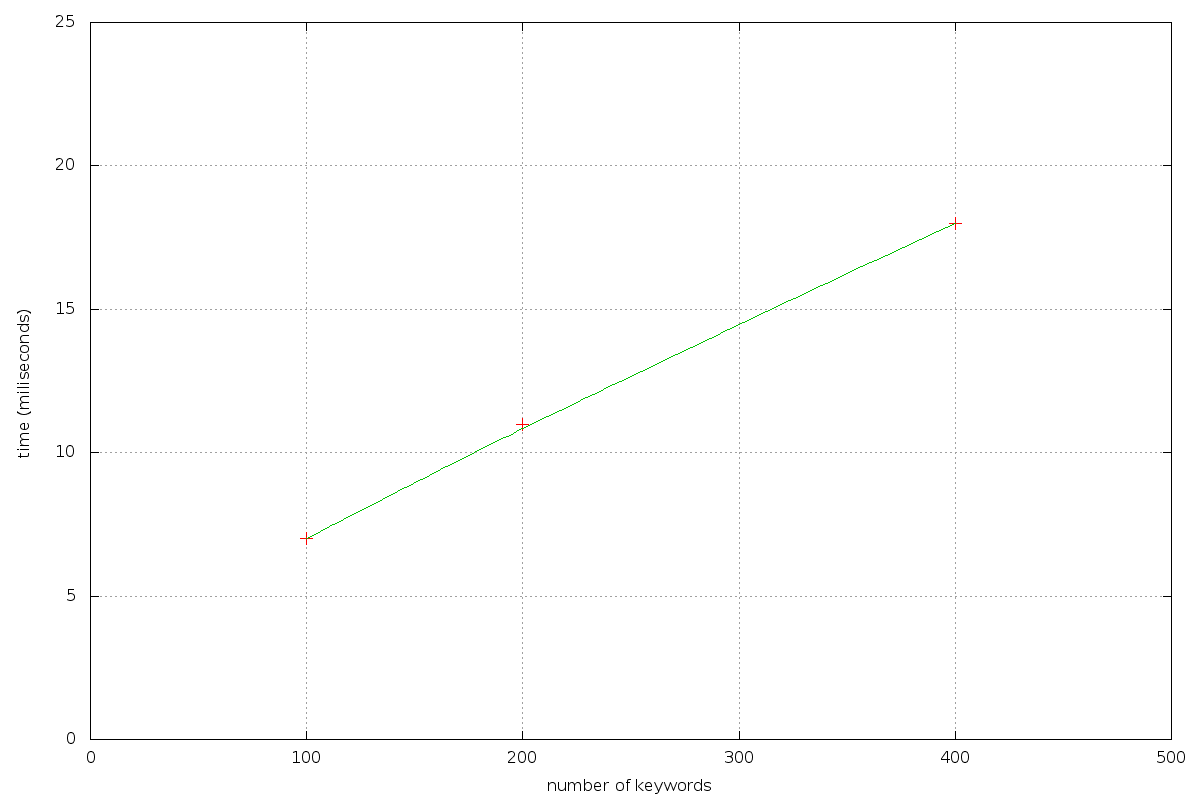
\includegraphics[width=\textwidth,height=!]{ahostatemachine}
  \end{center}
  \caption{Aho-Corasick state machine construction}
  \label{fig:ahostatemachine}
\end{figure} 

\begin{figure}
  \begin{center}
	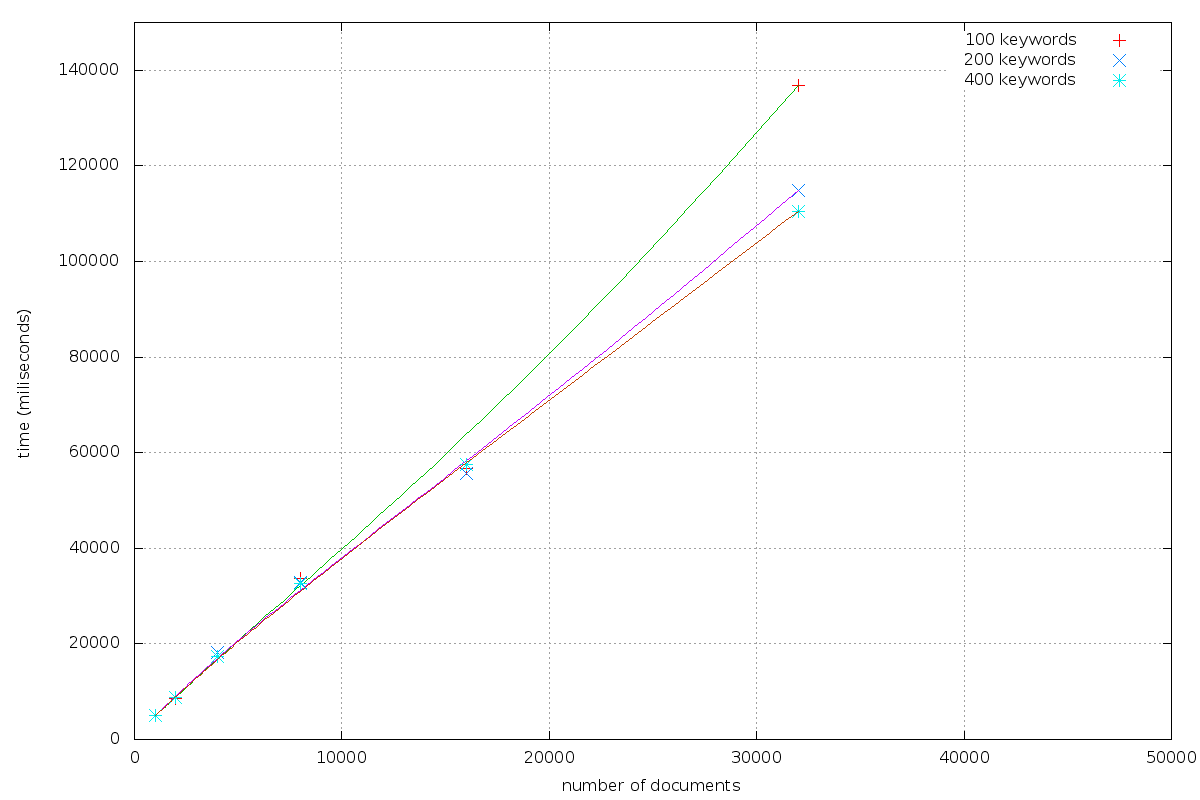
\includegraphics[width=\textwidth,height=!]{ahoscan}
  \end{center}
  \caption{Aho-Corasick state machine scanning}
  \label{fig:ahoscan}
\end{figure} 

\begin{figure}
  \begin{center}
	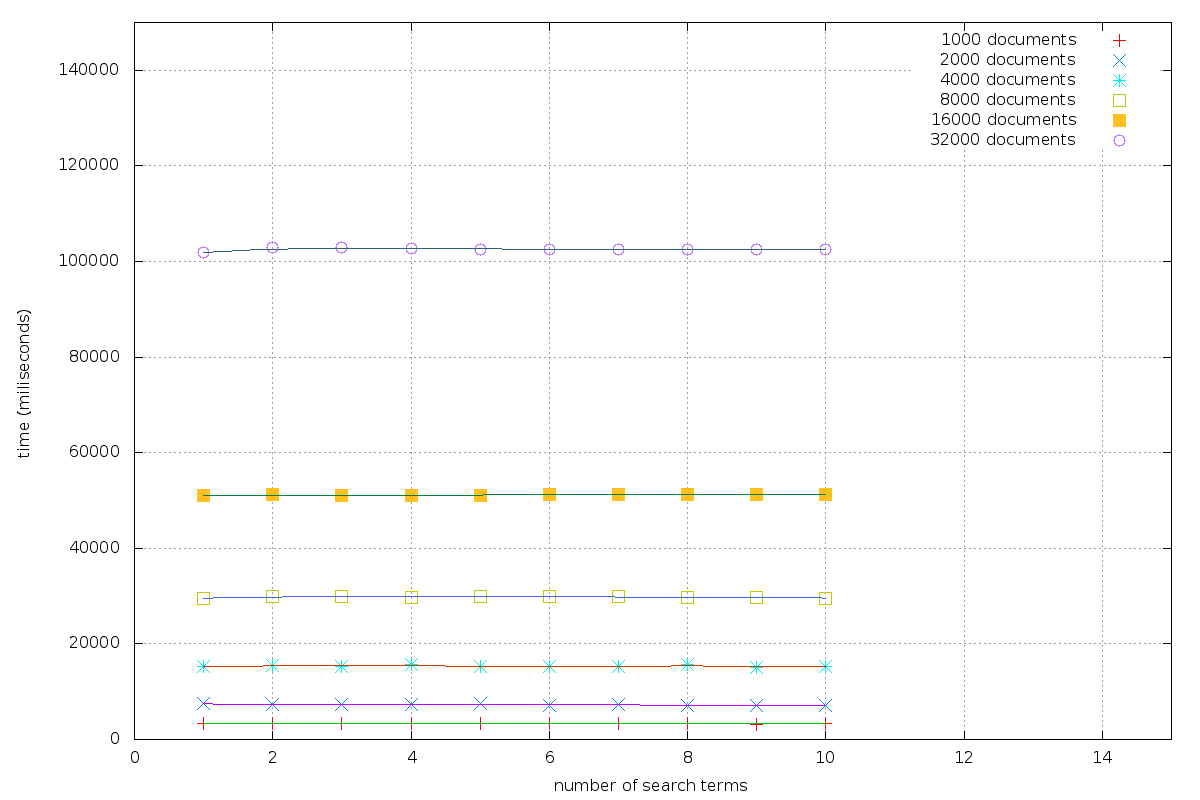
\includegraphics[width=\textwidth,height=!]{ahosearch}
  \end{center}
  \caption{Aho-Corasick state machine search}
  \label{fig:ahosearch}
\end{figure} 

%----------------------------------------
% Inverted Index
%----------------------------------------
\section{Inverted Index}
The program builds an \textit{inverted index} of a given corpus for
boolean search. The implementation is based on the techniques and
methods described in \cite{RefWorks:109}. A lexical scanner generator,
\textit{JFlex}\cite{RefWorks:112}, is used to generate a scanner to
construct a term index each document. The scanner is configured via a
set of regular expression macros to ignore a list of 430 stop
words. The term occurrences for each document are post-processed to
construct an inverted index mapping each term to a list of documents
containing the term.

The documents of the corpus are each stored in a disk file, named for
the identifier of the original blog extract. In an attempt to exploit
the fact that reading documents from disk is slower than state machine
scanning, the index creation process uses a thread pool to read and
parse multiple documents concurrently. By expanding the thread pool,
the implementation is able to achieve higher CPU utilization and
marginal improvements in index construction times. However, the limits
of the experiment platform did not accommodate increasing the pool
size to a point where the added complexity and synchronization
overhead were justified.


\subsection*{Implementation}
The \textit{inverted index} is generated by a Java
program. The only external dependency is on the Apache commons-cli
library for parsing commend line options. To that end, the program is
operated from the command line, taking options listed in table
~\ref{tab:invcommandline}.  
\\
\begin{table}[h]
  \centering
  \begin{tabular}{ |l|p{10cm}|} 
    \hline
    Option & Description \\ \hline
    -d \<arg\>  &  Document directory \\ \hline
    -p \<arg\>  &  Thread pool size. Default is 10 \\ \hline
    -h          &  Print help message \\ \hline
  \end{tabular}
  \caption{Command line options for inverted index implementation}
  \label{tab:invcommandline}
\end{table}
\\

The program implements various mechanism to facilitate
debugging. Throughout the code, log statements have been added using
the Java logging framework. The logging output is controlled for
individual classes via the \texttt{logging.properties} file which the
program reads on startup.

\begin{figure}
  \begin{center}
	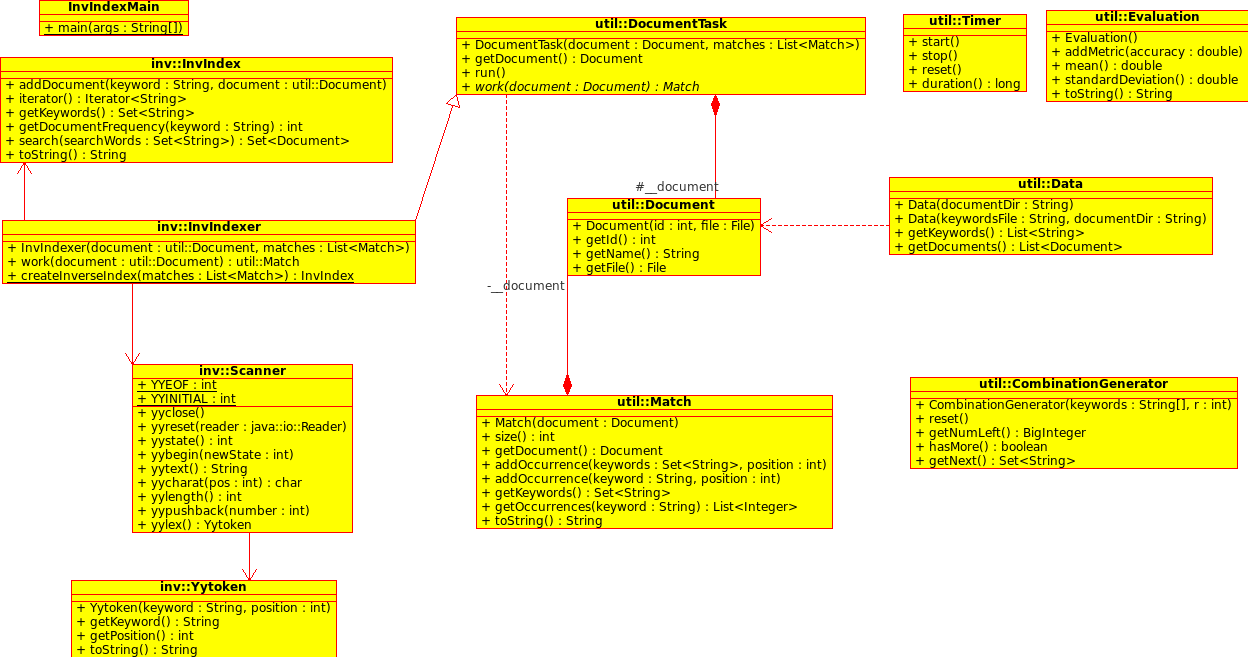
\includegraphics[angle=90,width=!,height=0.90\textheight]{invuml}
  \end{center}
  \caption{Inverted Index Implementation UML class diagram}
  \label{fig:invuml}
\end{figure} 

The implementation classes and their relationships are represented in a UML
class diagram in figure \ref{fig:invuml}. Following is a brief
description of each class:

\begin{itemize}
\item \textbf{CombinationGenerator:} this class generates the ${n
  \choose k}$ search term combinations required for the search
  evaluation. It borrows heavily from source code published by Michael
  Gilleland at Miriam Park Software.

\item \textbf{Evaluation:} a utility class for aggregating general
  test results and calculating means and standard deviations.

\item \textbf{InvIndexMain:} a driver class for the inverted index
  implementation. It performs the scanning tests and gathers data
  presented in this report. This class manages the thread pool used to
  parallelize the scanning process.

\item \textbf{InvIndexer:} manages the scanning of documents. It
  presents an interface suitable for use by the thread pool.

\item \textbf{Data:} utility class for reading blog and keyword files
  from the filesystem.

\item \textbf{Document:} encapsulates document attributes.

\item \textbf{DocumentTask:} abstract class which enforces an
  interface suitable for use by the thread pool. \texttt{InvIndexer}
  is a subclass.

\item \textbf{LogFormatter:} is a helper class to format log messages.

\item \textbf{Match:} maps a \texttt{Document} to a set of keywords
  that occur in the document and their position with the document.

\item \textbf{Scanner}: lexical scanner class generated by JFlex based
  on regular expression macros defining the stop word list and
  acceptable word boundaries.

\item \textbf{Timer:} utility class for collecting execution times.

\item \textbf{YyToken:} class returned by the \texttt{Scanner} when a
  token is found. This implementation bridges the gap between the JFlex
  tokens and the \texttt{Match} class used to generate the inverted
  index.
\end{itemize}

\subsection*{Results}
Various tests were conducted to characterize the performance of the
inverted index search algorithm:

\begin{itemize}
\item The time taken to construct the inverted index was measured for
  different sized corpora. The results of this test is shown in figure
  \ref{fig:invscan} and, as expected, indicate a linear relationship
  between index construction time and the size of the corpora.

\item The time taken to search for different numbers of keywords was
  measured over different sized corpora. A set of ten keywords was
  selected randomly and the the corpora searched for ${n \choose k}$
  enumerated combinations thereof to obtain an average for a
  particular keyword set size. The results of this test are shown in
  figure \ref{fig:invsearch}. If the results for one and ten search
  words are ignored, search times appear to be independent of the
  number of search terms and close to linear with respect to the size
  of the corpus. The unusual results for one and ten keywords warrant
  further investigation.
\end{itemize}


\begin{figure}
  \begin{center}
	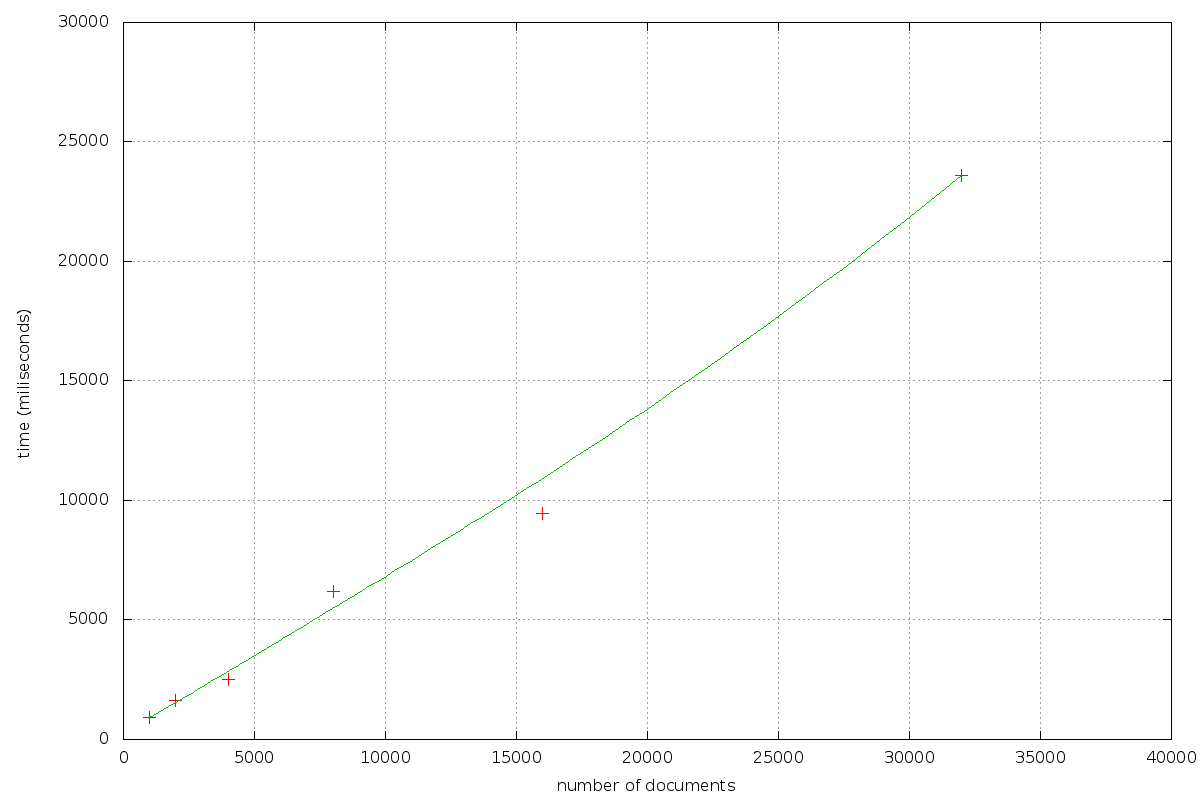
\includegraphics[width=\textwidth,height=!]{invscan}
  \end{center}
  \caption{Inverted index creation}
  \label{fig:invscan}
\end{figure} 

\begin{figure}
  \begin{center}
	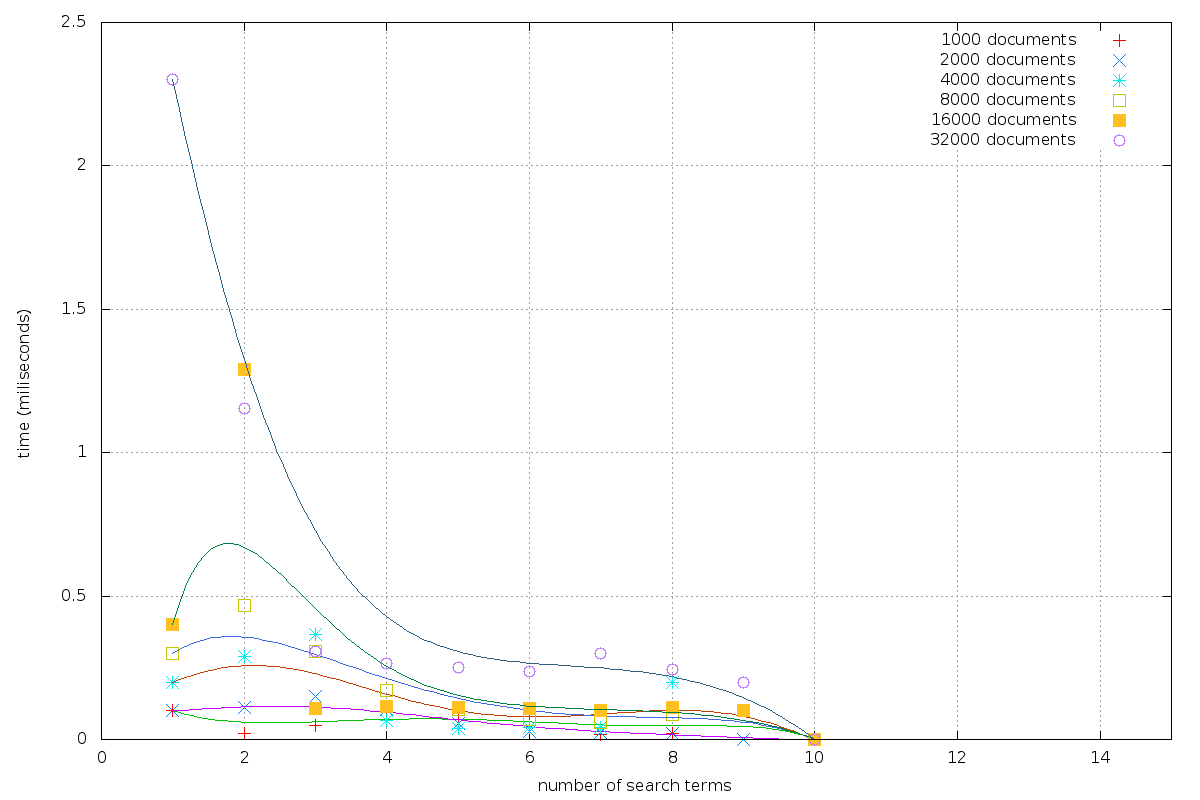
\includegraphics[width=\textwidth,height=!]{invsearch}
  \end{center}
  \caption{Inverted index search}
  \label{fig:invsearch}
\end{figure} 

%----------------------------------------
% Algorithm Comparison
%----------------------------------------
\subsection*{Algorithm Comparison}
\label{sec:algorithmcomparison}
All tests were run on a Dell laptop with an Intel Core Duo 2GHz
processor, 1GB RAM, running a 32 bit Linux 2.6.37 kernel. The Java
Virtual Machine used was version 1.6.0-24. 

Comparing corpus scan times for Aho-Corasick and inverted index
implementations, figures \ref{fig:ahoscan} and \ref{fig:invscan}
respectively, indicates that the inverted index scanner is
significantly faster than the Aho-Corasick state machine. Given that
the grammar supported by the JFlex-generated scanner is more expressive
than that of the Aho-Corasick state machine, one would expect results
to more comparable. Reviewing the source code of the generated scanner
indicates a compact and efficient implementation using packed data
structures to represent the internal state machine. In comparison, the
Aho-Corasick implementation is relatively unoptimized, closely
following the pseudo-code in \cite{RefWorks:103}.

Comparing search times for Aho-Corasick and inverted index
implementations, figures \ref{fig:ahosearch} and \ref{fig:invsearch}
respectively, indicates that the inverted index implementation has an
advantage of several orders of magnitude. The initial cost of creating
the inverted index is significantly larger than the creation of the
Aho-Corasick state machine however this cost is amortized over each
subsequent search. The Aho-Corasick implementation rescans the entire
corpus for each search, as opposed to a scan of the inverted index
alone. This exercise is a classic demonstration of the impetus behind
using indexed search techniques for large corpora.

%----------------------------------------
% Bibliography
%----------------------------------------
\bibliography{bibliography}
\bibliographystyle{IEEEannot}


%--------------------------------------------------
\end{document}
